\documentclass[11pt]{article}

\usepackage{geometry}
\usepackage{parcolumns}
\usepackage{amsmath}
\usepackage{siunitx}
\usepackage{titling}
\usepackage{xcolor}
\usepackage[T1]{fontenc}
\usepackage[variablett]{lmodern}
\usepackage{authblk}
\usepackage{helvet}
\usepackage{graphicx}
\usepackage{booktabs}

\usepackage{hyperref}
\definecolor{linkcolour}{rgb}{0.0,0.1,0.9}
\hypersetup{colorlinks,breaklinks,urlcolor=linkcolour, linkcolor=linkcolour, citecolor=black}

\usepackage[backend=biber,autocite = superscript]{biblatex}
\addbibresource{report.bib}

\graphicspath{ {./graphics/} }

\definecolor{light-grey}{gray}{0.90}

\newcommand*{\smallvttfamily}{%
      \footnotesize\fontencoding{T1}\fontfamily{lmvtt}\selectfont
  }
\newcommand*{\vttfamily}{%
      \fontencoding{T1}\fontfamily{lmvtt}\selectfont
  }

\title{An Analysis of The Fingerprintability of\\Web Traffic Through obfs4}
\author{James Houghton}
\affil[]{\textit{jth5zs@virginia.edu}}
\date{May 6, 2020}

\begin{document}

\maketitle

\begin{abstract}
Website Fingerprinting (WFP) attacks use information leaked by packet sequence information to detect which page a client might be visiting, even if they are connecting through an anonymizing proxy. They can achieve high accuracy when applied to the small set of Tor Hidden Services. Some WFP defenses have been proposed, but they are often difficult for Tor users to use. This can be because no online implementation exists, or the implementation is in an unrelated application. WFP defenses are most important for users living under oppressive governments, where bridges and pluggable transports may already be used. With this inspiration, we evaluate the existing packet size and timing obfuscation (IAT) modes in the obfs4 pluggable transport against some WFP attacks. We also implement a new IAT mode and evaluate its performance. We find that the existing obfuscation modes may not be adequate WFP defenses for small populations of monitored hidden services, but new IAT modes can be implemented to reduce information leakage.
\end{abstract}

\section{Introduction}
Internet anonymity systems attempt to prevent a server from learning the identities of users on the internet: an anonymity system may not know the identity of connecting clients, and any traffic observer will not be able to easily identify a particular user's traffic destination. People living in regimes with strict internet censorship may rely on these systems to communicate without obstruction. Tor~\cite{tor} is the largest and most popular example of such a system. Tor routes traffic through a series of relays such that no single host can resolve both the source and destination of any packets. Most Tor relays are listed publicly, making it easy for censors to block standard access to the Tor network. To get around this, non-publicly listed relays called \textit{bridges} are used. The use of bridges is often not enough to circumvent censorship, as censors can use deep packet inspection (DPI) to distinguish Tor traffic from other types of TCP traffic. In 2012, the Tor Project created the pluggable transport interface which lets clients and bridges connect to each other using a packet obfuscating proxy. Pluggable transports have, as of May 2020, allowed users in many countries with strict internet censorship like Iran, Russia, and China, to access the Tor network.

Several pluggable transports have been written. Among these, \textit{obfs4} is by far the most popular, with about 80\% of total PT users (Figure \ref{pts}).
\begin{figure}[tb] \label{pts}
    \centering
    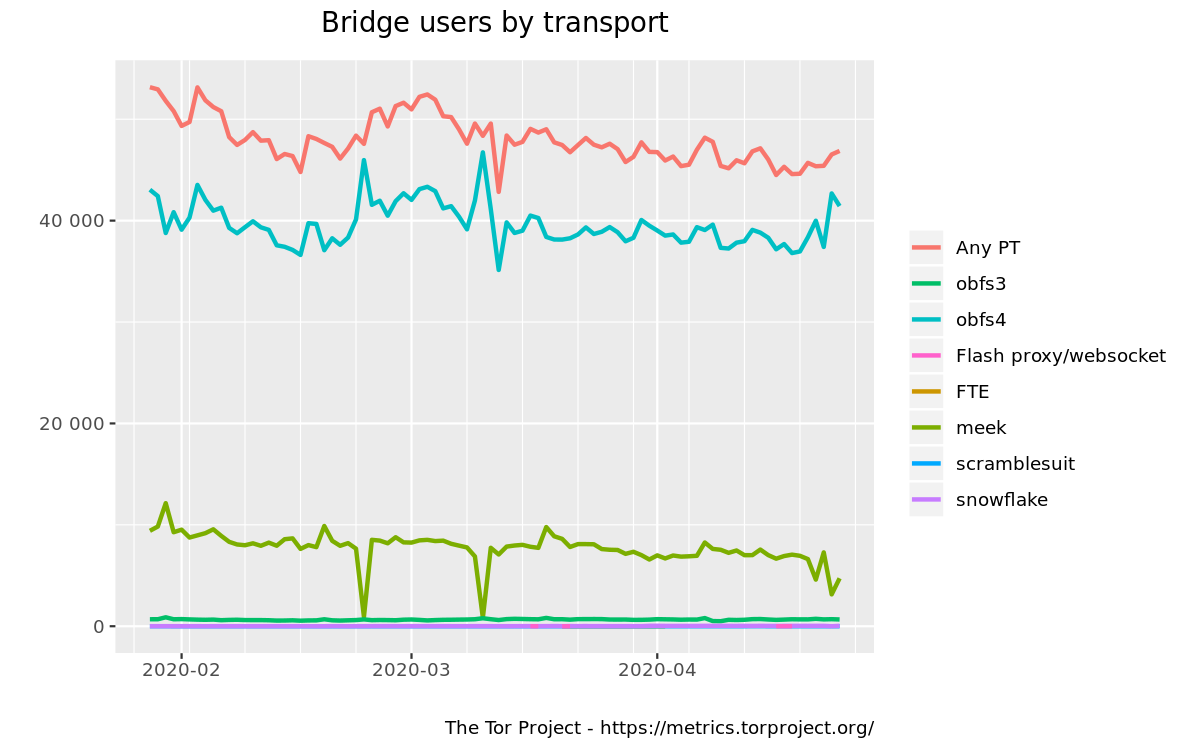
\includegraphics[scale=.6]{ptusage}
    \caption[]{Number of users by pluggable transport. From Tor Metrics.\footnotemark}
\end{figure}
\footnotetext{https://metrics.torproject.org/userstats-bridge-transport.html}
Obfs4 disguises Tor traffic as regular TCP traffic, preventing DPI from detecting that it's Tor traffic.

A user can still be de-anonymized through attacks like \textit{website fingerprinting}, where traffic patterns and other information leakage reveal the website a user is visiting. Such attacks are not very feasible on the whole web, but for the much smaller ecosystem of Hidden Services, website fingerprinting has shown to be effective~\cite{panchenko, wang}.
The variant of this attack discussed in this paper is a \textit{passive-observer website fingerprinting attack}, where the only information that is used comes from the packets sent between a client and a non-compromised guard or bridge. Anyone who sits between a client and the guard relay including internet service providers (ISPs) would be able to perform such an attack. If the ISPs are state-owned, that government would also be able to perform the attack. The types of governments that are likely to perform such an attack would have likely already blocked regular access to Tor requiring usage of a bridge and PT, probably obfs4. For this reason, in this report we analyze the fingerprintability of obfs4 traffic.

\section{Background}
\subsection{Tor}
Tor is an open-source anonymity system currently maintained by the Tor Project.\footnote{https://torproject.org} Tor uses onion routing, sending packets through a circuit of relays. Each relay in the circuit knows only the previous and next hop in the circuit. For a typical Tor connection to the internet, a circuit is comprised of three relays: the \textit{guard relay}, \textit{middle relay}, and \textit{exit relay}. The guard relay knows the identity of the client that is connecting to it, but does not know the final destination of any packets sent through it. To prevent Sybil attacks, the guard relay remains the same for many circuits, changing after a few months~\cite{sybil}. The middle relay proxies traffic from the guard to the exit relay. The exit relay performs the final decryption of the traffic and forwards it to the final destination, having no information about the originator of the packets.
This is basis for how the Tor network hides the identity of clients.

A Tor \textit{hidden service} (HS), or \textit{onion service}, is typically used to hide the identity of a server. HSes are anonymized in a similar fashion to clients; together, a six-hop circuit is created. To produce the six-hop chain, a client picks rendezvous point and builds a three-hop circuit with it (picking two additional relays for a total of three), while the hidden service builds a three-hop circuit to the rendezvous point (picking a total of three relays). Some hidden services that do not require anonymization may opt to operate as a \textit{single onion service}, where instead of creating a circuit to the RP, it directly connects to the RP, yielding a three-hop circuit instead of six. This mode only anonymizes the user but improves the speed of the connection. Hidden services are only accessible through the Tor network using its unique URL that will be referred to in this report as its \textit{onion link}, and there is quite a small population of them compared to all website on the internet.
Hidden services can operate completely privately, behaving as if they don't exist if a client attempts a connection without proper authorization. The number of hidden services operating this way are unknown.
Various services like OnionTree\footnote{https://oniontree.org} and Ahmia\footnote{https://ahmia.fi} catalog public hidden services. Most public hidden services serve webpages over HTTP, and these are the only types of services that can be considered for website fingerprinting.

\subsubsection{Bridges}
All guard, middle, and exit relays are publicly listed so that circuits can be generated through them. Internet censors can therefore easily block access to guard relays. To work around this limitation, \textit{bridge relays} (or just \textit{bridges}) are available for use with Tor. They are unlisted relays that take the place of guard relays in circuits. To use a bridge, a user must use resources created by the Tor Project like BridgeDB\footnote{https://bridges.torproject.org} or contact the Tor Project directly to get a list of a few bridges that can be used. This approach is not perfect; an adversary could still enumerate all or nearly all bridges, not only through services like this but also using port-scanning software. Indeed, several groups have been able list a significant number of bridges~\cite{troncoso}, but no attack has been so successful as to prevent bridge usage all together.

\subsubsection{Pluggable Transports}
Without obfuscation, bridge traffic looks very similar to guard relay traffic (i.e., Tor traffic), and it is generally possible to detect Tor traffic.
In 2012, the pluggable transport interface was created. A \textit{pluggable transport} is software that obfuscates traffic. A PT client runs on the Tor client host, and a PT server runs on the bridge. Instead of sending traffic straight to a bridge using the default onion routing (OR) protocol, a Tor client would send it to the local PT client which would send obfuscated packets over the network. When received by the bridge, the PT server interprets the packets and forwards the deobfuscated packets to the Tor instance running on the bridge. After this point, the regular onion routing scheme continues.

Pluggable transports can be created to bypass various modes of censorship. For example, if Skype traffic is unlikely to be blocked, one could use the SkypeMorph~\cite{skypemorph} PT to make Tor traffic look like Skype traffic.

The PTs that are currently deployed in the Tor Browser Bundle (TBB) are obfs4, meek, FTE, and ScrambleSuit (Figure \ref{pts}), with obfs4 making up approximately 80\% of all PT usage.

\subsubsection{Obfs4}
Obfs4 is a look-like-nothing transport that obfuscates traffic in such a way that the underlying protcol that is being used cannot be determined. Its current Go implementation\footnote{https://github.com/Yawning/obfs4}, as a part of obfs4proxy, can be used without Tor. In the context of Tor, obfs4 makes it difficult to determine that an end user is using Tor. It offers many protections against various attacks, including bridge enumeration attacks. Obfs4, as a low-latency PT, only has limited protection against website fingerprinting. It has various packet size and timing obfuscation options called IAT modes (from inter-packet arrival time). The goal of the analysis here is to determine if such protections are effective in the context of hidden services.

\subsection{Website Fingerprinting}
A website fingerprinting (WFP) attack uses information from traffic sent between a client and a server that allows an adversary to determine which website the client is visiting. The type of adversary considered in this report is one in which traffic between a user and non-compromised guard relay can be observed. This type of adversary is known as a \textit{passive observer}, as traffic is only being observed, not modified in any way. A real-world example of such an observer is a user's internet service provider. Passive-observer WFP attacks have been performed on Tor in the past. Panchenko et al~\cite{panchenko} used support vector machines to identify target webpages with an accuracy of 55\% for a population of 775 websites. Wang et al~\cite{wang} introduced the \textit{k-NN} attack which achieved a true positive accuracy of 85\% on 100 webpages while distinguishing them from 9000 unmonitored pages. Hayes and Danezis~\cite{hayes} introduced a random-forest-based attack that achieved a result of 85\% true positive rate for 30 hidden services and 100,000 unmonitored webpages.
The observed packet sequence generated by loading a particular hidden service is called a \textit{trace}. The packets sent between a client and a guard relay are almost always encrypted through either Tor's own hidden service end-to-end encryption or HTTPS. Although the contents of the packet are unknown, packet size, direction, retransmissions, and other metadata can still be observed. This information is the basis for fingerprinting attacks.

\subsubsection{Composite Features}
Although packet size and direction contain a lot of information, they become more useful when combined together to produce composite features. Examples of such features include the number of outgoing packets seen before another incoming packet is seen, the unique packets sizes seen during a connection, and the ratio of number of total incoming packets to the number of total outgoing packets. Using these features, website \textit{fingerprints} can be created for each trace created for a particular website.

\subsubsection{Homepage Fingerprinting}
In this analysis, we focus on \textit{homepage fingerprinting} of hidden services, where only homepages are considered for traffic analysis. However, because the Tor Browser does not save any sessions or login information when it is closed, many users will first be navigating to homepages before going to other pages, making homepage analysis quite powerful. For the rest of this report, website fingerprinting will refer to homepage fingerprinting.

\subsubsection{Fingerprinting Defenses}
Various defenses have been created to make website fingerprinting less feasible. These defenses are quite different, ranging from application-oriented like Wang's WalkieTalkie~\cite{walkietalkie} or Panchenko's decoy page technique~\cite{wang} to packet-oriented like the congestion-sensitive BuFLO server~\cite{buflo} or obfs4's own obfuscation modes. Many of these defenses are simulated and do not have online implementations. In other words, packet traces are morphed offline to simulate what would been produced by using the defense online. We implement an online fingerprinting defense into obfs4 based on DynaFlow and BuFLO and evaluate its performance.

\section{Implementation and Results}
The goal of a fingerprinting attack is to observe which hidden service a user is visiting if it is one that is being monitored. For a complete attack to be carried out, the following stages would likely be needed:
\begin{enumerate}
    \item Identify traffic of interest.
    \item Check that the traffic is HTTP/S.
    \item Identify where in a trace the page load of interest occurs.
    \item Check if the traffic is HS traffic, corresponding to a monitored service.
    \item If monitored, identify the service.
\end{enumerate}
None of these steps is easy, which is why website fingerprinting attacks are difficult to carry out.
All of the steps will be affected by the changes we are making in obfs4.
In this analysis we look only at the final step: identify a page when it is monitored. In other words, we have a closed-world scenario where we know all the sites a user could possibly be visiting.
Other works have been successful in both the closed- and open-world scenarios~\cite{hayes, wang, panchenko}.
The code written to perform our website fingerprinting attack is available on GitHub: \href{https://github.com/jamesthoughton/obfs4-fp}{https://github.com/jamesthoughton/obfs4-fp}.

\subsection{Implementation as Additional IAT Mode}
Although obfs4 is not designed to prevent website fingerprinting, its Go implementation already contains three IAT modes that attempt to slightly hinder it. The IAT (inter-packet arrival time) modes modify packet sizes and can delay packets by a random amount of time. The first IAT mode disables it. We will call this mode IAT0. The second IAT mode (so-called ``regular'', IAT1) obfuscates packet timing, sending groups of packets at a random time between 0 and 100 milliseconds. The distribution of the random time is configurable. The third IAT mode (so-called ``paranoid'', IAT2) obfuscates both packet timing and size, adding random padding to each packet, and sending groups of packets at a random time. Although the regular IAT mode tries to maintain good performance, the paranoid mode does not. A fourth mode (IAT3) was implemented, attempting to match the performance of the paranoid mode while providing better protection against fingerprinting. The code for this implementation is public here: \href{https://github.com/jamesthoughton/obfs4}{https://github.com/jamesthoughton/obfs4}.

An obfs4 server and client do not need to run the same IAT modes. In other words, a server can obfuscate the packets it sends to the user while the user does not modify the packets it sends to the server. This type of asymmetric configuration is not considered in this analysis as it is atypical.

\subsubsection{The Dispatcher: Packet Timing and Size Obfuscation}
IAT3 uses a queue-based packet system to obfuscate timing. A dispatcher thread was added to obfs4 that send out packets every 50 milliseconds. This sending interval is the first of the configuration parameters that can be used. Every 50 milliseconds, 8 AEAD frames are sent. Authenticated encryption with associated data (AEAD) frames contain data that will be encrypted and sent over the network. The number of full AEAD frames sent is correlated but not equal to the number of TCP packets sent. The number of AEAD frames sent per dispatch is another configurable parameter. If there is enough queued data to fill all frames, all the data would be sent. If there is not enough data, the AEAD frames are filled with data to pad out the size. This has the effect of always sending some TCP packets over the network. Because the data is only sent every 50 milliseconds, packet timing is obfuscated. This approach limits the total bandwidth per connection. The size of the underlying packets in this case will be entirely obfuscated. To save bandwidth, if there is no data to send, nothing is sent.

\subsubsection{Data Multiplication: Content Size Obfuscation}
In order to obfuscate packet size, we used a packet multiplier. In other words, for each byte that is about to be enqueued, we enqueue an additional number of bytes proportional to the number of bytes enqueued. For example, if we are sending 500 bytes and the packet multiplier is currently $1.5$, we will enqueue 1250 bytes. The data multiplier is resampled every 10 minutes, but this is configurable as well as its distribution. We reasoned that it would be more effective to resample the data multiplier no more than a few times per connection, and resampling it on the order of minutes should provide reasonable efficacy. This approach avoids some caveats that come with other content size obfuscation approaches: it does not use constant bandwidth, and it does not rely on databases of content to emulate. However, this approach can incur quite a large bandwidth overhead. For example, using a uniform distribution from $0$ to $2$ yields an average bandwidth overhead of 100\%.

\subsubsection{All Configurable Parameters}
With these two aspects of the new IAT mode discussed, we summarize the configurable parameters:
\begin{enumerate}
    \item The dispatch interval (default 50ms)
    \item The number of AEAD frames sent on each dispatch event (default 8)
    \item The data multiplier distribution (default $\text{Uniform}[0-2]$)
    \item The data multiplier resampling frequency (default 10 minutes)
\end{enumerate}

\subsection{Producing Fingerprints}
To produce fingerprints for a particular webpage, it needs to be downloaded several times. While fetching webpages, the packets need to be sniffed (observed). After collecting traces for a particular website, the metadata and other information can be extracted from each trace to produce data for use in classification.
\subsubsection{Fetching Traces}
We used the browser automation library Selenium that had been extended to work with the Tor Browser\footnote{https://github.com/webfp/tor-browser-selenium}. We used Tor Browser version 9.0.1 with Tor version 0.4.2.6 for the client. To actually fetch the packets, we used tcpdump, filtering for packets that were either sent or received by our bridge. The Tor version used on the bridge was Tor 0.4.2.7.

To get a list of the hidden services to be fingerprinted, OnionTree was crawled for valid onion links, where one link was chosen for listed service. This yielded approximately 160 working links. Of these links, several are SecureDrop sites for different news organizations. SecureDrop has a very similar fingerprint for each news organization, so code is included to filter them. The list of 160 working links was shortened to 80. Over the course of this work, 8 hidden services stopped working, so the final list contained 72 onion links.

Before any onion links were tried, Tor and obfs4 were started on both the bridge and the client. These instances were not stopped or restarted until all traces were downloaded. This means that the same Tor circuit was re-used for multiple traces. Because Tor circuits are regenerated every few minutes, no two traces of the same HS will have used the same circuit. Each onion link was attempted once and given 90 seconds to fully load. If the page didn't fully load in 90 seconds, the traces would be marked as bad, and that onion link would be put on a list of onions to retry. After every onion is tried once, the all onions on the retry list is attempted again. If onions fail a second time, they are placed on a set of once-failing onions. This entire process is repeated many times. If 40 traces per HS are needed, this process will be repeated 40 times.

Failing onions slow down the fetching process significantly. To save time, an optimization was added: if a once-failing onion failed twice a second time in a row, it became a twice-failing onion. If it fails another two attempts, it is presumed dead and no longer attempted. This only occurs if an onion fails 6 back-to-back attempts, where each subsequent attempt comes at least several minutes after the previous.

This process was used to create 40 traces for obfs4 running with IAT0, IAT2, and IAT3 with default parameters. We also created an additional 15 traces per onion for IAT0, IAT1, IAT2, IAT3 with default parameters, and IAT3 with a data multiplier distribution that was uniform from 0 to 5.

\subsubsection{Feature Extraction}
For each trace, we extract various features for fingerprinting.
Based on previous website fingerprinting attacks we decided on the following features:
\begin{enumerate}
    \item Total outgoing packets
    \item Total incoming packets
    \item Total packets
    \item Total outgoing bytes
    \item Total incoming bytes
    \item Total bytes
    \item Total outgoing bytes as a proportion of the total
    \item Total incoming bytes as a proportion of the total
    \item Total retransmissions
    \item Final packet timestamp
    \item Unique packet sizes of at most 1500 bytes
    \item Packet directions for the first 5000 packets
\end{enumerate}
Trace parsing was done using the Python library pypcapfile\footnote{https://github.com/kisom/pypcapfile}. Each trace has its features extracted, and all the traces are placed into a CSV file for classification.

\subsection{Evaluating Fingerprintability}
With a filled CSV file containing the extracted features from every trace for a particular run, they are labeled with their hidden service name. Similar to Hayes' k-FP attack~\cite{hayes}, we use a random forest classifier on the data. The data was split for training and testing: 70\% for training and 30\% for testing. We used a random forest with 500 estimators, and the fitting was repeated 20 times with the best result saved.

\subsubsection{Results for 72 Monitored Sites}
The two sets of fingerprints were collected for the entire set of 72 monitored services: 40 iterations per service for IAT0, 2, and 3, and an additional 15 iterations per service for IAT0, 1, 2, 3, and 3 with a maximum data multiplier of 5 (designated IAT3-5).

\begin{figure}[ht]
    \centering
    \begin{tabular}{|l|r|r|}
        \hline
        IAT Mode & Average Accuracy (15 iterations) & (40 iterations) \\
        \hline
        IAT0  & $11.26 \pm 0.07$\% & $17.73 \pm 0.06$\%\\
        IAT1  & $15.12 \pm 0.11$\% & -\\
        IAT2  & $15.39 \pm 0.07$\% & $18.07 \pm 0.06$\%\\
        IAT3  & $ 9.19 \pm 0.08$\% & $12.81 \pm 0.09$\%\\
        IAT3-5& $ 6.02 \pm 0.07$\% & -\\
        \hline
    \end{tabular}
    \caption[]{Performance of IAT0, IAT1, IAT2, IAT3, and IAT3-5 on all 72 hidden services, 70/30\% training/test split. There error reported is the 68.3\% confidence interval after 20 fits. There are no results for IAT1 and IAT3-5 for 40 iterations because those traces were not generated.}
\end{figure}

Some immediate observations from the results are that the accuracy of all tested configurations are somewhat similar. Although much better than guessing, a real attack could not be carried out with this classification method. However, the results are useful for comparing the relative strengths of the defenses.

IAT1 and 2 appear to not improve security, in fact seemingly increase fingerprintability. We are not sure why this is the case. IAT3 with the default maximum data multiplier of 2 decreases fingerprintability over IAT0. With IAT3-5, fingerprintability is even further decreased, likely due to the fact that many more websites with vastly differing content sizes are harder to distinguish from each other.

Another key observation is that accuracy goes up slightly as more traces are included. In a widely shared dataset generated by Wang~\cite{wang}, 90 traces per monitored service is used.

\subsection{Bandwidth Overhead}
Tor is designed to be a low-latency anonymity network, and in keeping with that choice, pluggable transports should not excessively slow down clients' connections. To get an idea of the performance penalty for using each IAT mode, we measured time between the first and last packet received for each page load. This approximates the total time to load a page to within a few seconds.
\begin{figure}[tb]
    \centering
    \begin{tabular}{|l|c||r|r|r|r|r|r|}
        \hline
        HS & IAT Mode & Min & 1st Qu. & Median & Mean & 3rd Qu. & Max \\
        \hline
        \texttt{facebookcorewwwi} & IAT0 & 10.26 & 13.32 & 15.63 & 21.07 & 19.19 & 90.42 \\
        \texttt{facebookcorewwwi} & IAT3 & 19.62 & 22.41 & 25.81 & 28.11 & 28.32 & 73.59 \\
        \texttt{rougmnvswfsmd4dq} & IAT0 & 4.79 & 6.36 & 8.10 & 9.16 & 10.10 & 43.53 \\
        \texttt{rougmnvswfsmd4dq} & IAT3 & 6.88 & 9.99 & 11.63 & 13.79 & 12.98 & 90.53 \\
        \hline
    \end{tabular}
    \caption[]{Full page load times in seconds for Facebook and Tor Metrics. The numbers for IAT3 may be a slight overestimate, as it includes a few seconds for browser startup.}
\end{figure}
\begin{figure}[tb]
    \centering
    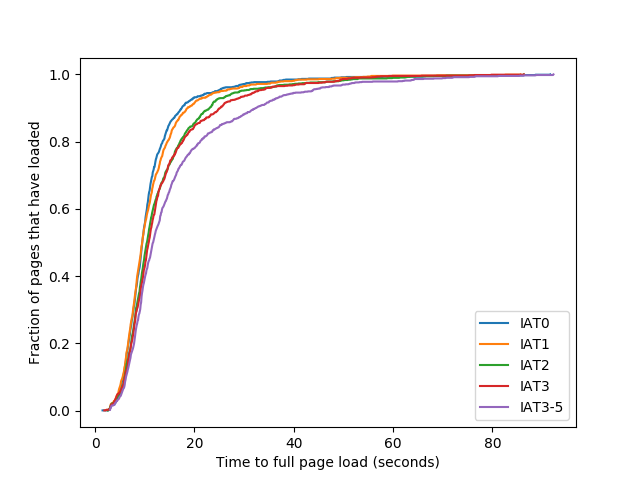
\includegraphics[scale=.45]{bw-allpages}
    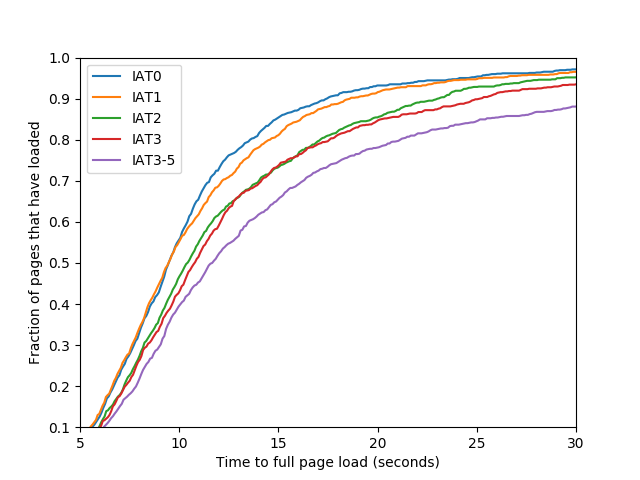
\includegraphics[scale=.45]{bw-allpages-trunc}
    \caption[]{Plots of the fraction of all pages that have loaded after a certain time period. The left plot shows all 90 seconds, where the right plot shows only data for page loads between 5 and 30 sceonds, where there is the most variation.}
\end{figure}
\begin{figure}[tb]
    \centering
    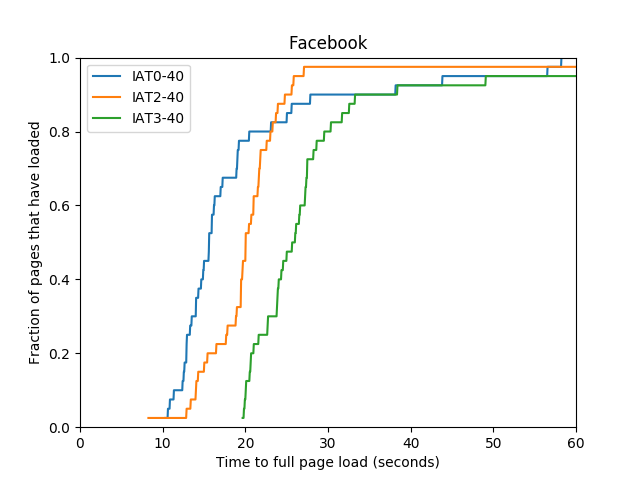
\includegraphics[scale=.45]{bw-fb}
    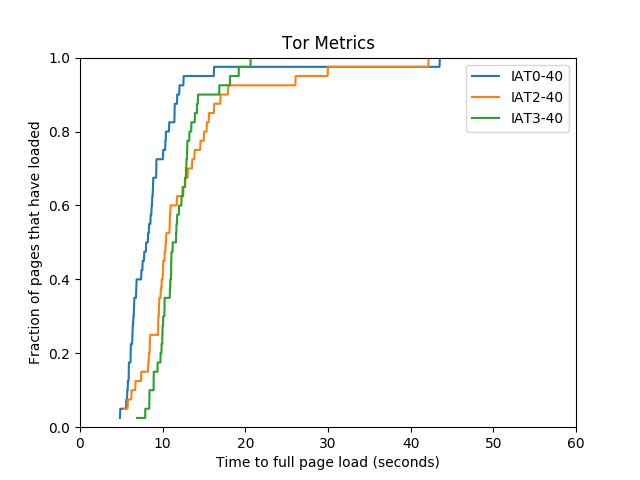
\includegraphics[scale=.45]{bw-metrics}
    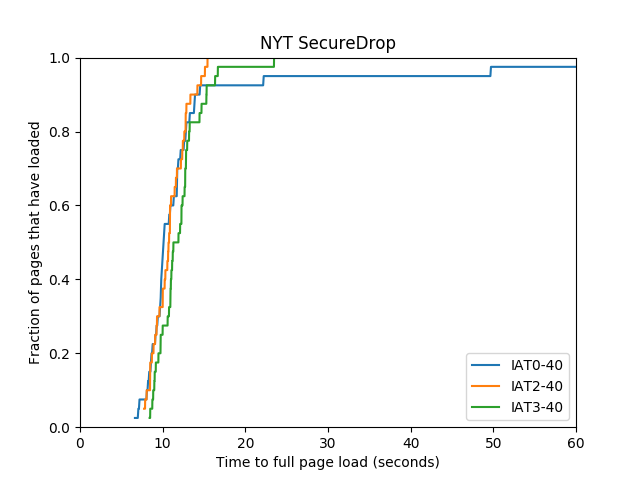
\includegraphics[scale=.45]{bw-nyt}
    \caption[]{Page load time plot for the Facebook, New York Times' SecureDrop, and Tor Project's Tor Metrics hidden services. New York Times' SecureDrop bandwidth is representative of all SecureDrop hidden services. These plots were created from the 40-iteration traces, as 15 iterations are not enough for conclusive results.}
\end{figure}

From these results, we can see that IAT3 is nearly as fast as IAT2. IAT3-5 is quite slow, nearly doubling page load time. This is expected, as on average, it is sending 3.5 times more traffic than IAT1. We can look at the data more finely by looking at individual services. We use Facebook as a representative large page, Tor Metrics as medium-sized, and New York Times' SecureDrop as small. We deduce that about 10 seconds of the page load time is somewhat fixed, and only the additional time above that is affected by the PT in use. We see that Facebook through IAT2 takes about 25\% more time than IAT0, and IAT3 takes about 50\% more time than IAT0. We conclude that despite IAT2 and IAT3 yielding similar page load latencies on average, large pages load more slowly through IAT3.

These data were collected with a high-bandwidth, low-latency internet connection to the bridge. The bandwidth results may be significantly affected by the quality of the connection to the bridge.

\section{Discussion}
\subsection{Important Artifacts}
Although the fingerprinting accuracy achieved in this research does not compete with the state-of-the-art, several useful artifacts were produced:
\begin{enumerate}
    \item Code to find onion services, download traces, and perform feature extraction.
    \item An IAT mode in obfs4 that hinders website fingerprinting, even if the improvement is marginal.
\end{enumerate}
\subsection{Improvements and Future Work}
Our experimentation has not been able to achieve classification accuracy results similar to the state-of-the-art. It should be possible to create enough packet traces to use other attacks, and although this was explored during this project, the results could not be replicated properly. Additional experimentation is necessary to draw strong conclusions about the fingerprintability of obfs4 web traffic.

To carry out a successful fingerprint attack, one needs to perform many steps that are not done here. This includes being able to tell the difference between regular traffic and Tor HS traffic. Our obfs4 IAT3 traffic fingerprint may be unique enough to distinguish it from other kinds of TCP connections, making it easier to narrow down possible Tor usage. This could also be true for the other IAT modes. If this were possible, there would be little to no need to identify an HTTP/S connection earlier.

Additional study into how the various configurable parameters affect the fingerprintability of IAT3 is also another avenue to continue this research.

\printbibliography

\end{document}
